\documentclass{beamer}
\mode<presentation>
{
	\usetheme{Antibes}
}
\usepackage[utf8]{inputenc}
\usepackage[english]{babel}

\usepackage{tikz}
\usetikzlibrary{graphs, positioning, arrows, matrix}
\usepackage{sansmathaccent}
\pdfmapfile{+sansmathaccent.map}
\usepackage{amssymb,latexsym,amsmath,amscd,amsthm, mathtools,stmaryrd, hyperref, enumitem, array, cleveref}

\title{Supersingular Isogeny Diffie-Hellman}
\author{Valeriia Kulynych}
\institute{Université de Toulon}
\date{May 25th, 2018}
\begin{document}

\begin{frame}
	\titlepage
\end{frame}

\begin{frame}
	\frametitle{Outline}
	\tableofcontents
\end{frame}

\section{Supersingular Elliptic Curves}

\begin{frame}
	\begin{definition}
		An \alert{elliptic curve} is a pair $(E, O)$, where $E$ is a curve of genus 1 and $O \in E$.
	\end{definition}
	
	Composition law is defined as follows:
		Let $P, Q \in E$, $L$ be the line connecting $P$ and $Q$ (tangent line to $E$ if $P = Q$), and $R$ be the third point of intersection of $L$ with $E$. Let $L'$ be the line connecting $R$ and $O$. Then $P \oplus Q$ is the point such that $L'$ intersects $E$ at $R, O \ \text{and} \ P \oplus Q$.

\end{frame}

\begin{frame}
\begin{figure}
	\hfill
	%% 
	\begin{center}
	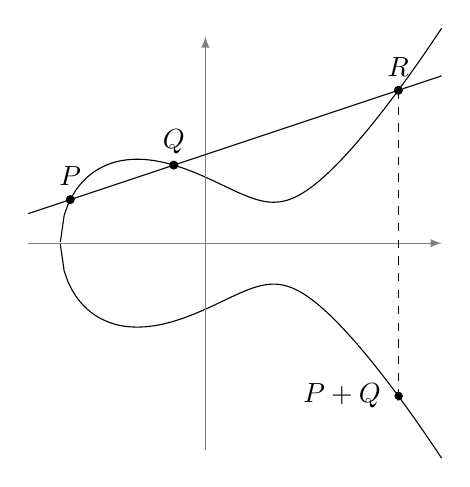
\begin{tikzpicture}[domain=-2.4566:4,samples=100,yscale=3/8,xscale=3/4]
		\draw plot (\x,{sqrt(\x*\x*\x-4*\x+5)});
		\draw plot (\x,{-sqrt(\x*\x*\x-4*\x+5)});
	
		\draw[thin,gray,-latex] (0,-7) -- (0,7);
		\draw[thin,gray,-latex] (-3,0) -- (4,0);
	
		\draw (-3,1) -- (4,8/3+3);
		\begin{scope}[every node/.style={draw,circle,inner sep=1pt,fill},cm={1,2/3,0,0,(0,3)}]
			\node at (-2.287980,0) {};
			\node at (-0.535051,0) {};
			\node at (3.267475,0) {};
		\end{scope}
		\begin{scope}[every node/.style={yshift=0.3cm},cm={1,2/3,0,0,(0,3)}]
			\node at (-2.287980,0) {$P$};
			\node at (-0.535051,0) {$Q$};
			\node at (3.267475,0) {$R$};
		\end{scope}
	
		\draw[dashed] (3.267475,3.267475*2/3+3) -- (3.267475,-3.267475*2/3-3) 
			node[draw,circle,inner sep=1pt,fill] {}
			node[xshift=-0.1cm,anchor=east] {$P+Q$};
	\end{tikzpicture}
	\hfill
	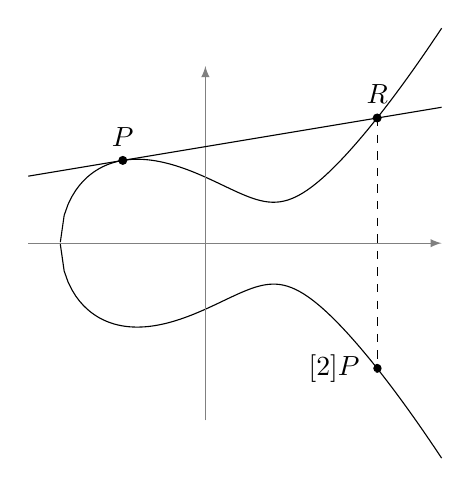
\begin{tikzpicture}[domain=-2.4566:4,samples=100,yscale=3/8,xscale=3/4]
		\draw plot (\x,{sqrt(\x*\x*\x-4*\x+5)});
		\draw plot (\x,{-sqrt(\x*\x*\x-4*\x+5)});
		
		\draw[thin,gray,-latex] (0,-6) -- (0,6);
		\draw[thin,gray,-latex] (-3,0) -- (4,0);
	
		\def\c{3.269524}
		\def\P{-1.398674}
		\def\R{2.908459}
		\draw (-3,-1+\c) -- (4,4/3+\c);
		\begin{scope}[every node/.style={draw,circle,inner sep=1pt,fill}, cm={1,1/3,0,0,(0,3.269524)}]
			\node at (\P,0) {};
			\node at (\R,0) {};
		\end{scope}
		\begin{scope}[every node/.style={yshift=0.3cm},cm={1,1/3,0,0,(0,3.269524)}]
			\node at (\P,0) {$P$};
			\node at (\R,0) {$R$};
		\end{scope}
	
		\draw[dashed] (\R,\R/3+\c) -- (\R,-\R/3-\c) 
			node[draw,circle,inner sep=1pt,fill] {}
			node[xshift=-0.1cm,anchor=east] {$[2]P$};
	\end{tikzpicture}

		\hfill
		\strut
	
	\end{center}
	
	\caption{An elliptic curve defined over $\mathbb{R}$, and the geometric
		representation of its group law.}
	\label{fig:weierstrass}
\end{figure}
\end{frame}


\end{document}
